\documentclass[12pt, a4paper,twoside,titlepage]{article}
\usepackage[left=3.5cm,top=2cm,right=3cm,includehead]{geometry}

%% ¡¡ Modificar !! %%
\newcommand{\grado}{Grado en Ingeniería de la Ciberseguridad}

\newcommand{\pregunta} {CTF}
\newcommand{\asignatura}{Metodologías de Desarrollo Seguro}
\newcommand{\curso}{Curso 2021-2022}
\newcommand{\githubCI}{\href{https://github.com/Skayara/practica-ctf-mds}{Skayara/practica-ctf-mds}}
\newcommand{\autorA}{Clara Contreras Nevares}

\usepackage[round]{natbib}
\let\cite\citep

%%%%%%%%%%%%%%%%%%%%%%% Paquetes (no modificar)
\usepackage[utf8]{inputenc}
\usepackage[spanish,es-lcroman,es-tabla]{babel}
\usepackage[T1]{fontenc}
\usepackage[pdftex]{graphicx}
\usepackage{mathtools}
\usepackage{mathptmx}
\usepackage{amsmath}
\usepackage{amssymb}
\usepackage{enumitem}
\usepackage{minted}
\usepackage{caption}
\usepackage[justification=centering]{caption}
\setlength\abovecaptionskip{0.5em}
\setlength\belowcaptionskip{-0.25em}
 \usepackage[figuresright]{rotating}
 \usepackage{booktabs}
\usepackage{multirow}
\usepackage{xltabular}
\usepackage{longtable}
\usepackage{pdflscape}
\usepackage{afterpage}
\usepackage{relsize}
\usepackage{color}
\usepackage{xcolor}
\usepackage{booktabs}
\usepackage{subcaption}
\definecolor{linkcolor}{RGB}{52,59,144}
\definecolor{Comment}  {RGB}{169,082,044}
\definecolor{Bluedark} {RGB}{0,0,180}
\definecolor{Bluelight}{RGB}{070,100,250}
\definecolor{Browndark}{rgb}{0.2,0.2,0.2}
\definecolor{gray}{rgb}{0.6,0.6,0.6}
\usepackage{tikzpagenodes}
\usepackage[linesnumbered,ruled]{algorithm2e}
% \usepackage{algpseudocode}
\usepackage[hidelinks]{hyperref}


%%%%%%%%%%%%%%%%%%%%%%% Estilo de código
\usepackage{textcomp}
\usepackage{bold-extra}
\usepackage{listings}
\usepackage{titlesec}
\usepackage{minted}
% Definition of \subparagraph emulating that of the standard classes
% \titleformat{\subparagraph}[runin]
%     {\normalfont\normalsize\bfseries}{\thesubparagraph}{1em}{}
% \titlespacing*{\subparagraph}{\parindent}{3.25ex plus 1ex minus .2ex}{1em}

% Definition of \subparagraph starting new line after heading
\titleformat{\subparagraph}
    {\normalfont\normalsize\bfseries}{\thesubparagraph}{1em}{}
\titlespacing*{\subparagraph}{\parindent}{3.25ex plus 1ex minus .2ex}{.75ex plus .1ex}
\newcommand{\code}{\lstinline[
  language={},
  columns=fullflexible,
  basicstyle=\color{Browndark}]
}
\lstdefinestyle{Default}{
  basicstyle = \relsize{-1}\ttfamily\color{Bluelight},
  keywordstyle=\color{Bluedark},
  stringstyle=\color{Browndark},
  commentstyle = \color{Comment},
  numberstyle=\tiny\color{Bluedark},
  xleftmargin=0.5cm,
  numbers=left,
  basewidth = 0.48em,
  columns=fullflexible,
  breaklines,
  breakatwhitespace=true,
  moredelim=*[s][\color{Browndark}]{[}{]},
  moredelim=[s][\color{Bluedark}]{\{}{\}},
  mathescape = true,
  upquote = true,
  inputencoding=utf8,
  extendedchars=true,
  showstringspaces=false,
  literate      =        % Support additional characters
  {á}{{\'a}}1  {é}{{\'e}}1  {í}{{\'i}}1 {ó}{{\'o}}1  {ú}{{\'u}}1
  {Á}{{\'A}}1  {É}{{\'E}}1  {Í}{{\'I}}1 {Ó}{{\'O}}1  {Ú}{{\'U}}1
  {ä}{{\"a}}1  {ë}{{\"e}}1  {ï}{{\"i}}1 {ö}{{\"o}}1  {ü}{{\"u}}1
  {ñ}{{\~n}}1  {Ñ}{{\~N}}1  {¿}{{?`}}1  {¡}{{!`}}1
  {\\\%}{{\textbackslash\%}}2  {~}{{\raisebox{0.5ex}{\texttildelow}}}1
  {<-}{{$\gets\ $}}1
}
\lstdefinestyle{Python}{style=Default, language=Python}
\lstdefinestyle{Java}{style=Default, language=Java}
\lstdefinestyle{C}{style=Default, language=C}
\lstdefinestyle{HTML}{style=Default, language=HTML}
\lstdefinestyle{Unity}{style=Default, language=[Sharp]C}
\lstdefinestyle{Latex}{style=Default, language=[LaTeX]TeX}
\lstdefinestyle{VHDL}{style=Default, language=VHDL}
%% Selecciona el estilo por defecto: Python, Unity, Latex, Default, ...
\lstset{style=VHDL}

%%%%%%%%%%%%%%%%%%%%%%% Estilo de páginas
\definecolor{mordantred19}{rgb}{0.68, 0.05, 0.0}
\usepackage{fancyhdr}
\pagestyle{fancy}
\fancyhf{}
\setlength{\headheight}{15.2pt}
%\renewcommand{\chaptermark}[1]{\markboth{\uppercase{#1}}{}}
\renewcommand*{\headrulewidth}{0pt}
\fancyhead[EL]{ \textsf{\relsize{-1}{\grupo\ }} \hrulefill }
\fancyhead[OR]{ \hrulefill \textsf{\relsize{-1}{\ \nouppercase\pregunta} } }
\fancyfoot[C]{\thepage}
\hypersetup{
    colorlinks=true,
    linkcolor=red,
    urlcolor=grey,
    citecolor=mordantred19,
    pdftitle={Práctica 2}
    }

%%%%%%%%%%%%%%%%%%%%%%%%%%%%%%% Portada
\renewcommand*{\maketitle}{%
\begin{titlepage}
  \pagestyle{plain}

  \begin{center}
    \vspace*{-4em}
    
\includegraphics[scale=.3]{Figuras/urjc.jpg}\\
    \vspace*{2em}
    \textsc{\LARGE Escuela Técnica Superior\\de Ingeniería Informática}\\
    \vspace*{2em}
    \textsc{\Large \grado}\\  
    \vspace*{\fill}
    \textbf{\LARGE \pregunta\\}  
    \vspace*{2em}
    \textsc{\large \asignatura\\}
    \vspace*{.5em}
    \textsc{\large \curso\\}  
    \vspace*{4em}\vspace*{\fill}
    \textbf{\large \githubCI\\} 
    \vspace*{4em}\vspace*{\fill}
    {%
      \large
      \begin{tabular}{rl}
        \textbf{\autorA}\\
      \end{tabular}
    }
  \end{center}
  
\end{titlepage}
}

\sloppy

%%%%%%%%%%%%%%%%%%%%%%%%%%%%%%% Inicio del documento
\begin{document}

\maketitle

%%%% Inicio Artículo %%%%
\thispagestyle{plain}

\section{Adivina}

Nos encontramos con el siguiente enunciado de reto:\\

\textbf{La ruleta, la lotería, el bingo... Muchos juegos de azar, por supuesto siempre trucados a favor de la casa. ¿Existirá alguna forma de asegurar nuestras ganancias?}\\

Se nos proporciona una página web con la siguiente interfaz, así como su código fuente:\\

\begin{figure}[H]
    \centering
    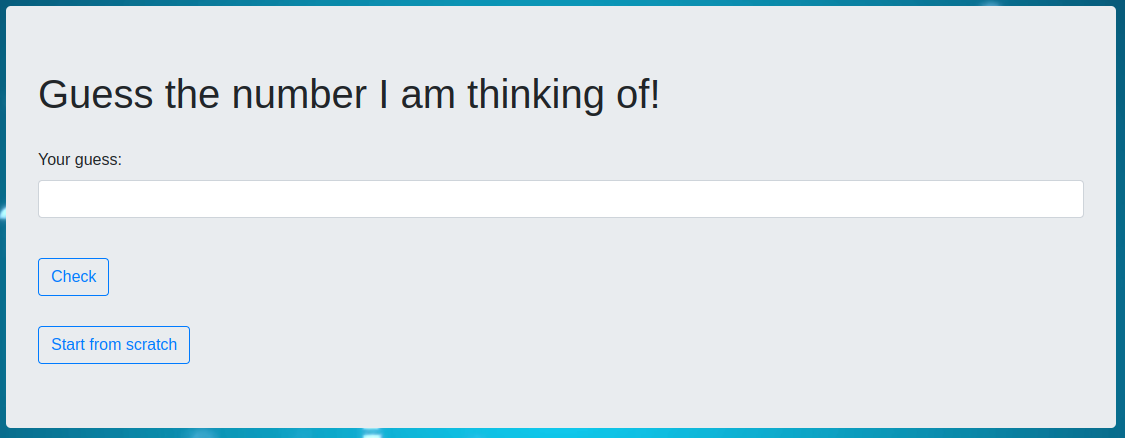
\includegraphics[width=1\linewidth]{Figuras/Adivina/1.png}
    \caption{Interfaz principal}
    \label{fig:adivina}
\end{figure}

Nos percatamos de que al introducir un número al azar:

\begin{figure}[H]
    \centering
    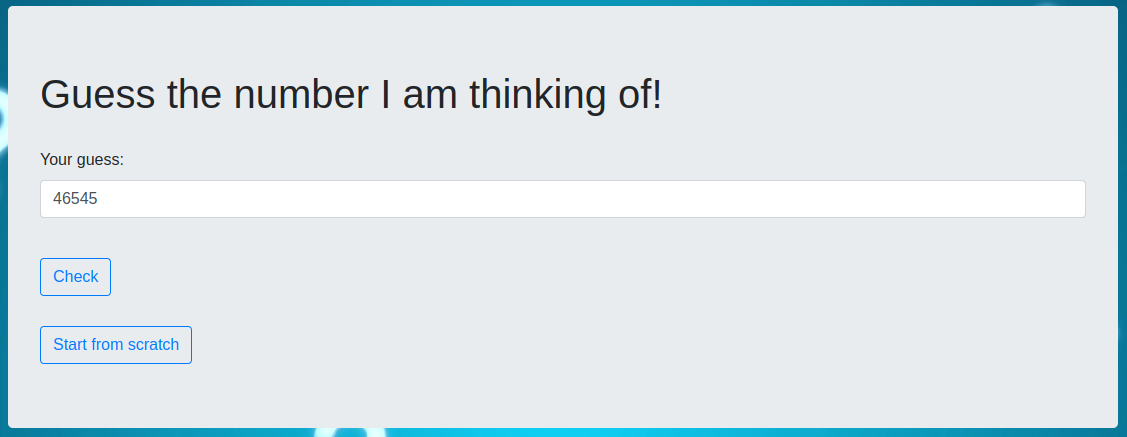
\includegraphics[width=1\linewidth]{Figuras/Adivina/2.png}
    \caption{Entrada random}
    \label{fig:adivina}
\end{figure}

Al hacer click en \emph{Check}, obtenemos un número diferente al introducido:

\begin{figure}[H]
    \centering
    
\includegraphics[width=1\linewidth]{Figuras/Adivina/3.png}
    \caption{Check de número random}
    \label{fig:adivina}
\end{figure}

Si miramos el código fuente de la página, podemos ver que en el HTML se envía el número introducido con un método POST a /check:

\begin{minted}[linenos]{html}
<form method="POST" action="/check">
    <div class="form-group">
        <label for="number">Your guess:</label><br>
        <input class="form-control" type="number" min="0" id="number" 
        name="number"><br>
    </div>
    <button type="submit" class="btn btn-outline-primary">
        Check
    </button>
</form>
\end{minted}

Observamos el método /check en el código proporcionado:

\begin{minted}[linenos]{java}
@PostMapping("/check")
ModelAndView checkToken(@RequestParam int number, ModelAndView mv, 
    HttpServletRequest request){
    
    var session = request.getSession(true);
    boolean correct = tokenManager.isValidToken(session, number);
    if(correct){
        mv.addObject("flag", flag);
        mv.setViewName("correct");
    } else {
        var usedTokens = tokenManager.getUsedTokens(request
            .getSession(true));
        mv.addObject("usedTokens", usedTokens);
        mv.setViewName("tryHarder");
    }
    return mv;
}
\end{minted}

Vemos que hace uso de una función llamada \emph{getUsedTokens}, por lo que procedemos a analizar dicha función:

\begin{minted}[linenos]{java}
public Iterable<Integer> getUsedTokens(HttpSession session){
    String id = session.getId();
    var usedTokens = clients.get(id).usedTokens;
    log.info(String.format("Returning used tokens for client \%s --> 
    \%s", id, usedTokens));
    return usedTokens;
}
\end{minted}

Devuelve el contenido de un set de tokens, no nos aporta información, por lo que analizamos otra función utilizada en el método \emph{checkToken}:

\begin{minted}[linenos]{java}
public boolean isValidToken(HttpSession session, int token){
    String id = session.getId();
    clients.computeIfAbsent(id, ClientTokenState::new);
    boolean result = clients.get(id).isValidToken(token);
    log.info(String.format("Validating token for client %s got %s 
    --> %s", id, token, result));
    return result;
}
\end{minted}

En este método aparece el \emph{ClientTokenState}, miramos cómo se genera dicha variable analizando el constructor:

\begin{minted}[linenos]{java}
private static class ClientTokenState {
        final String clientIP;
        final Queue<Integer> usedTokens;
        int currentToken;
        Random random;

        ClientTokenState(String clientIP) {
            this.clientIP = clientIP;
            this.usedTokens = new ConcurrentLinkedQueue<>();
            this.random = new Random(System.currentTimeMillis());
            this.currentToken = random.nextInt(1_234_000_000);
        }

        boolean isValidToken(int token){
            boolean check = token == currentToken;
            usedTokens.add(currentToken);
            currentToken = random.nextInt(1_234_000_000);
            log.info(String.format("Token -> %s", currentToken));
            return check;
        }
    }
}
\end{minted}

La parte que nos interesa es el constructor de \emph{ClientTokenState} con una ip:

\begin{minted}[linenos]{java}
ClientTokenState(String clientIP) {
    this.clientIP = clientIP;
    this.usedTokens = new ConcurrentLinkedQueue<>();
    this.random = new Random(System.currentTimeMillis());
    this.currentToken = random.nextInt(1_234_000_000);
}
\end{minted}

Con esto vemos cómo se genera un número aleatorio en base al tiempo en milisegundos en el que es generado, por lo que podemos probar a invertir el proceso y conseguir así la semilla.\\

Se desarrolla el siguiente código en java:

\begin{minted}[linenos]{java}
import java.util.Random;

public class adivina {
    public static void main(String[] args) {
        int a = 540267208;
        int cont = 0;
        long currentToken;
        Random random;
        long time = System.currentTimeMillis();

        int i = 0;
        while (i<180000){
            random = new Random(time - i);
            currentToken = random.nextInt(1_234_000_000);
            if (a == currentToken) {
                cont = cont + 1;
            }
            if (cont == 1) {
                System.out.println(random.nextInt(1_234_000_000));
                System.exit(0);
            }
            i ++;
        }
    }
}
\end{minted}

En la variable \emph{a} colocamos el valor que nos ha devuelto la web como número usado. Utilizamos un bucle while para "volver atrás en el tiempo", buscando el momento en el que se generó la variable a y su semilla.\\

Una vez obtenida la salida, probamos a introducir el número en la web:\\

\begin{figure}[H]
    \centering
    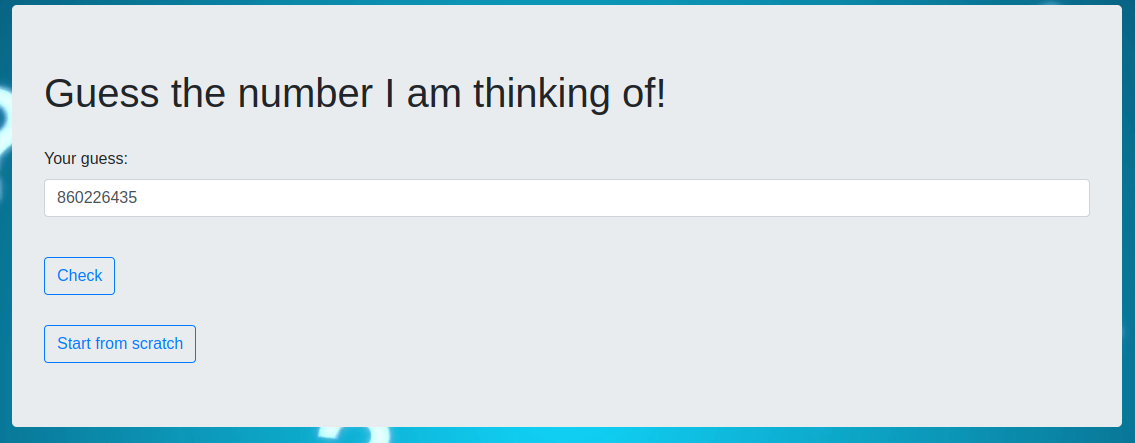
\includegraphics[width=1\linewidth]{Figuras/Adivina/4.png}
    \caption{Introduciendo la salida del código}
    \label{fig:Adivina}
\end{figure}

Al hacer click en \emph{check}, obtenemos la flag:

\begin{figure}[h]
    \centering
    
\includegraphics[width=1\linewidth]{Figuras/Adivina/Flag.png}
    \caption{Flag}
    \label{fig:Adivina}
\end{figure}

\newpage

\section{Optimizer}

Nos encontramos con el siguiente enunciado de reto:\\

\textbf{Nuestro nuevo becario del grupo GRAFO lleva semanas trabajando en un nuevo software de optimización, pero a diferencia de nuestros expertos alumnos parece que no sigue mucho las mejores prácticas de programación, especialmente si nuestro código es público en GitHub...}

Además, se nos proporciona el código en forma de zip.\\

Con el comentario de que el código está público en GitHub intuímos que tiene vulnerabilidades detectables por SonarCloud, por lo que procedemos a subirlo a SonarCloud. En el apartado de vulnerabilidades observamos lo siguiente:\\

\begin{figure}[H]
    \centering
    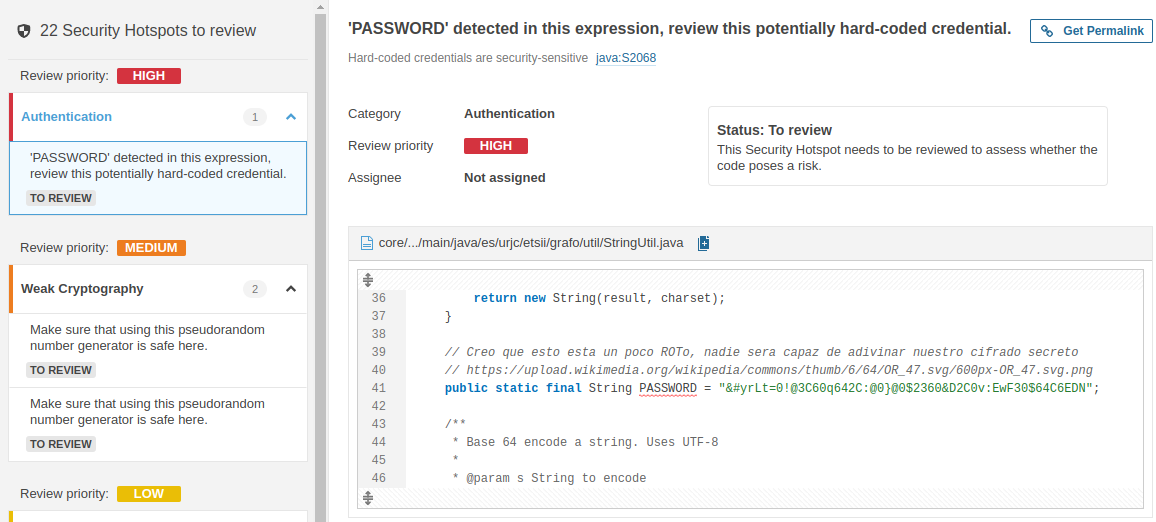
\includegraphics[width=1\linewidth]{Figuras/Optimizer/1.png}
    \caption{Vulnerabilidad Optimizer}
    \label{fig:Optimizer}
\end{figure}

En los comentarios vemos que pone \emph{ROTo}, buscamos cifrados ROT y vemos que hay varios. Si seguimos el enlace también hallado en comentarios, obtenemos la siguiente imagen:

\begin{figure}[H]
    \centering
    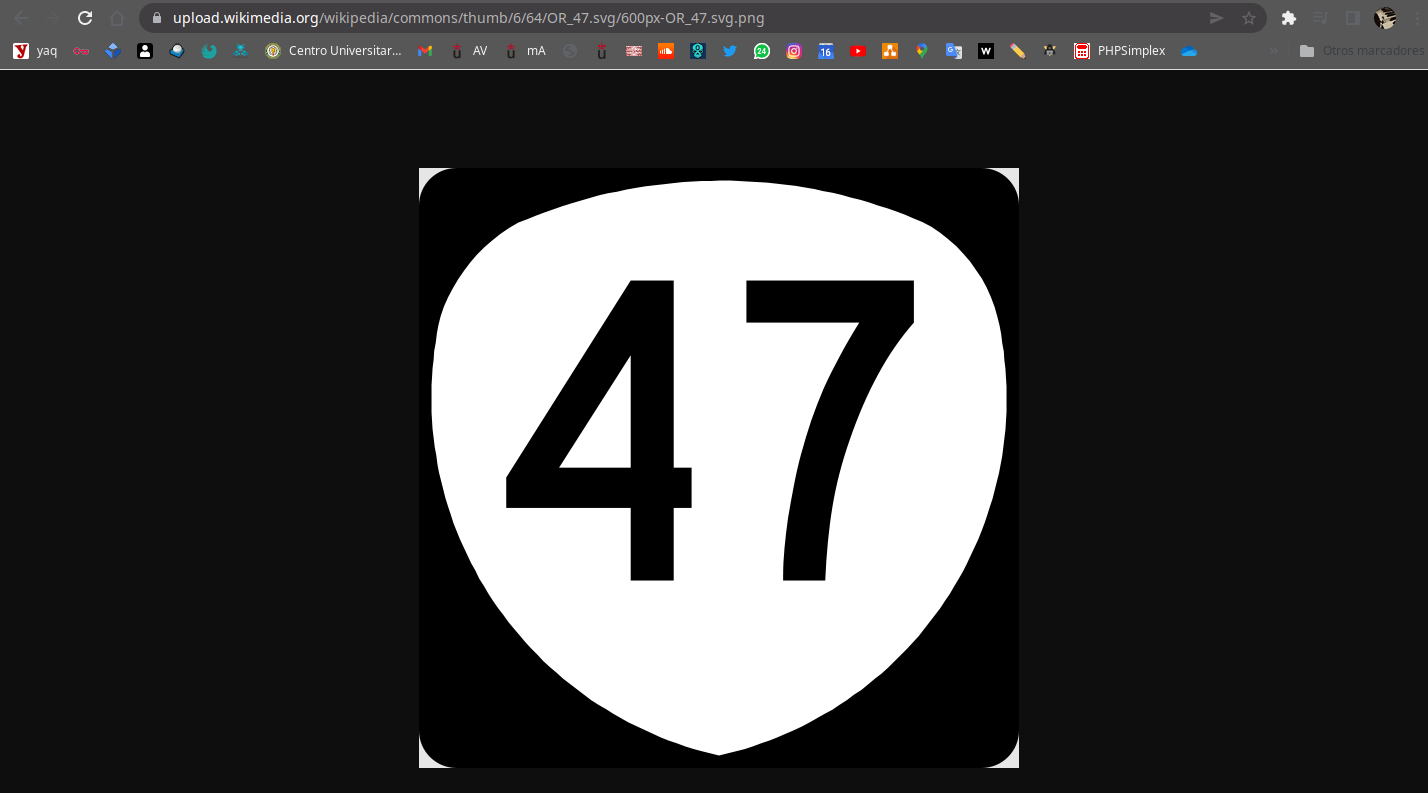
\includegraphics[width=1\linewidth]{Figuras/Optimizer/2.png}
    \caption{Enlace comentarios}
    \label{fig:Optimizer}
\end{figure}

Esta imagen nos da la pista del tipo de cifrado ROT, decodeamos el texto de la variable \emph{PASSWORD}:

\begin{figure}[H]
    \centering
    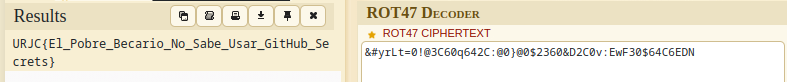
\includegraphics[width=1\linewidth]{Figuras/Optimizer/3.png}
    \caption{Flag}
    \label{fig:Optimizer}
\end{figure}

\newpage

\section{La calculadora}

Nos encontramos con el siguiente enunciado:\\

\textbf{El nuevo becario se ha encargado de programar una nueva calculadora para nuestro sistema de cobro en caja. Antes de desplegarla en producción, nos han pedido verificar que cumple unos mínimos de calidad. Debemos comprobar el correcto funcionamiento de la "calculadora segura" que nos ha proporcionado. En caso de detectar comportamiento erróneo, arreglalo y comprueba que el test funciona correctamente. En concreto, es necesario verificar la siguiente funcionalidad:
\begin{itemize}
    \item En caso de intento de división entre 0, debe tirar ArithmeticException.
    \item Debe protegerse contra Overflows de forma correcta: por ejemplo la multiplicacion de dos numeros positivos nunca puede dar un numero negativo.
    \item En caso de overflow, tirar ArithmeticException.
    \item Debe generar números aleatorios de forma correcta, en el limite pedido.
    \item Debe detectar correctamente cuando un numero es par y cuando un numero es impar.
    \item Debe emitir mensajes de log si ha sido configurada para ello.
\end{itemize}
Una vez hayas completado los tests, puedes comprobar si has terminado de arreglar la calculadora utilizando el siguiente servicio:\\ http://ctf-vulnerable.numa.host:8085. Puede que tenga alguna flag para ti :D\newline
El código fuente de este reto está disponible en el Aula Virtual.}

\vspace{6mm}
\subsection{Multiply}

Para obtener el resultado de forma correcta en forma de long, hay que haces un casting previo a cada variable:

\begin{minted}[linenos]{java}
public long multiply(int a, int b){
    log("Multiply %s * %s", a, b);
    long result = (long)a * (long)b;
    return result;
}
\end{minted}

\vspace{6mm}
\subsection{Mod}

Los problemas encontrados al hacer el módulo entre dos números son en caso de que el segundo sea un 0, por lo que lanzamos una excepción en ese caso. Además hacemos uso de la función floorMod de Math, que lleva a cabo un módulo más seguro en caso de números negativos:

\begin{minted}[linenos]{java}
public int mod(int a, int b){
    log("%s mod %s", a, b);
    if( b == 0)
        throw new ArithmeticException();
    return Math.floorMod(a, b);
}
\end{minted}

\vspace{6mm}
\subsection{IsOdd}
Añadimos el log y utilizamos la función floorMod:
\begin{minted}[linenos]{java}
public boolean isOdd(int a){
    log("Comprobar si %s es impar", a);
    return Math.floorMod(a, 2) == 1;
}
\end{minted}

\vspace{6mm}
\subsection{IsEven}
Seguimos el mismo proceso que con isOdd:

\begin{minted}[linenos]{java}
public boolean isEven(int a){
    log("Comprobar si %s es par", a);
    return Math.floorMod(a, 2) == 0;
}
\end{minted}

\vspace{6mm}
\subsection{GetRandomNumber}
Generamos un número aleatorio de la clase Random, siempre inferior al número máximo de la clase Integer.

\begin{minted}[linenos]{java}
public int getRandomNumber(){
    log("Generating rnd");
    return new Random().nextInt(Integer.MAX_VALUE);
}
\end{minted}

\vspace{6mm}
\subsection{GetRandomNumber con máximo}
Seguimos el proceso previo, pero añadiendo la comrpbación de que el máximo introducido no es mayor al número máximo de la clase Integer y en ese caso estableciendo el máximo en el número pasado como argumento.
\begin{minted}[linenos]{java}
public int getRandomNumber(int bound){
    log("Generating rnd with bound %s", bound);
    if (bound > Integer.MAX_VALUE)
        throw new IllegalArgumentException("Invalid range");
    return new Random().nextInt(bound);
}
\end{minted}

\vspace{15mm}

Subimos el archivo corregido y obtenemos la flag:
\begin{figure}[H]
    \centering
    \includegraphics[width=1\linewidth]{Figuras/Calculadora/Flag.png}
    \caption{Flag}
    \label{fig:my_label}
\end{figure}

\newpage

\section{Agenda 1}

Nos encontramos con el siguiente enunciado:\\

\textbf{Tenemos una nueva agenda de contactos, de capacidad algo limitada... ¿Podrás recuperar la flag?\\
nc ctf-vulnerable.numa.host 9993}

Además, se proporciona el código de dicha agenda.\\

Procedemos a analizar los puntos de entrada. El primero se halla en la función \emph{add\_contact}, en la línea 4, la entrada se almacena en la variable \emph{pos} y posteriormente se comprueba que el contenido de dicha variable esté en el rango adecuado, por lo que no es un punto de entrada:
\begin{minted}[linenos]{c}
void add_contact(){
    printf("En que posicion de la agenda quieres almacenar el 
    numero?\n");
    int pos;
    scanf("%d", &pos);

    if(pos >= SIZE || pos < 0){
        printf("Posicion invalida! Que tramas?\n");
        return;
    }
    printf("Introduce el numero (Solo lee 8 chars): ");
    scanf("\%8s", agenda[pos]);
}
\end{minted}

También se prueba a almacenar cadenas concretas en el array \emph{agenda[]} y leerlas después, sin obtener resultados.
\\
Se procede a analizar el siguiente punto de entrada hallado en la función \emph{show\_contact}, línea 4:
\begin{minted}[linenos]{c}
void show_contact(){
    printf("Que contacto quieres recuperar? Indica su posicion en la agenda.");
    int pos;
    scanf("%d", &pos);

    if(pos >= SIZE){
        printf("Posicion invalida! Que tramas?\n");
        return;
    }

    printf("El numero de la posicion %d es %s\n", pos, agenda[pos]);
}
\end{minted}

En este caso sólo se comprueba que la posición introducida sea menor que el tamaño total, lo que incluye números negativos.\\
Probamos a introducir números negativos para leer contactos, hasta llegar al -6, donde obtenemos la flag:

\begin{figure}[H]
    \centering
    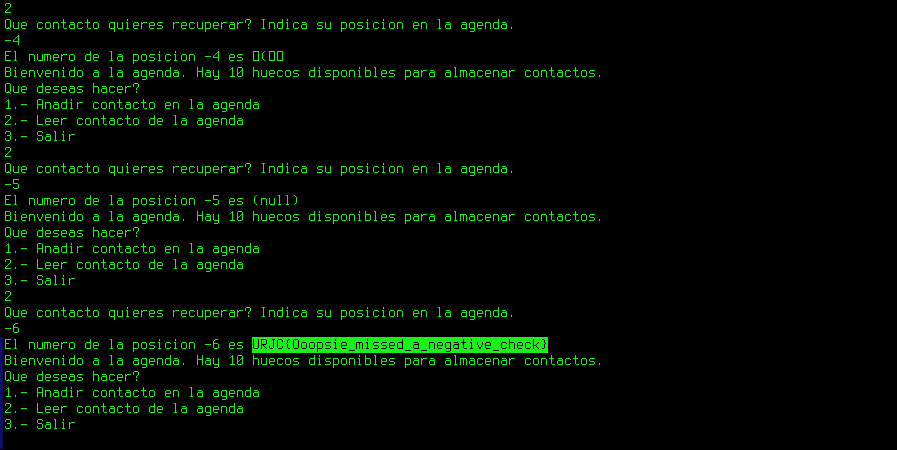
\includegraphics[width=1\linewidth]{Figuras/Agenda1/Flag.png}
    \caption{Flag}
    \label{fig:my_label}
\end{figure}

\newpage

\section{Caja Negra}

Nos encontramos con el siguiente enunciado:\\


\textbf{Existen muchas formas de comprobar si un PIN de 8 dígitos es correcto, ¿podrás fuzzearlo?}\\

Además se proporciona el código ofuscado del archivo .c.\\

Hacemos uso de la herramienta opensource afl, para ello compilamos el archivo .c con afl-gcc y modificamos el script por defecto hallado en el repositorio de github afl-demo:


\begin{minted}[linenos]{bash}
#!/bin/bash
AFL=/home/sky/AFL
export CC=$AFL/afl-clang
export CXX=$AFL/afl-clang++
mkdir -p aflbuild \
&& cd aflbuild \
&& cmake .. \
&& make \
&& $AFL/afl-fuzz -i ../testcases -o ../findings ./../a.out
\end{minted}

Siendo a.out el binario compilado del archivo .c proporcionado.\\

Ejecutamos el script hasta que hallamos un crash:

\begin{figure}[H]
    \centering
    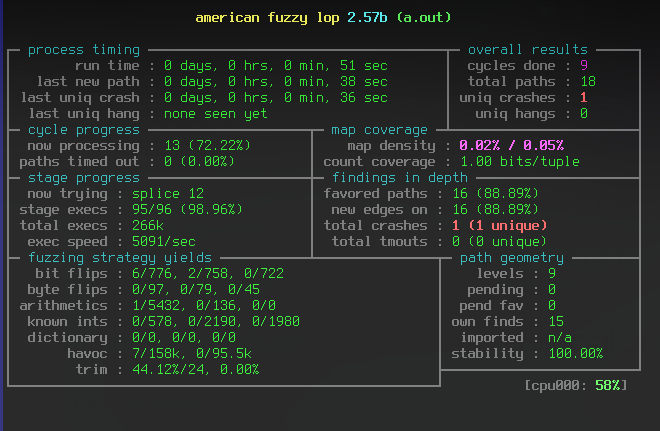
\includegraphics[width=140mm]{Figuras/Caja Negra/Analisis.png}
    \caption{Analisis}
    \label{fig:my_label}
\end{figure}

Leemos dicho crash almacenado en la carpeta findings/crashes y obtenemos el pin de 8 dígitos que estábamos buscando:

\begin{figure}[H]
    \centering
    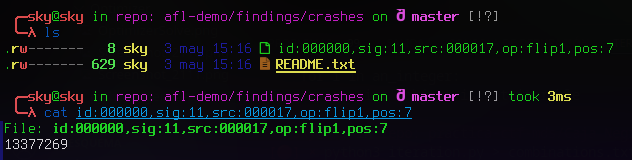
\includegraphics[width=140mm]{Figuras/Caja Negra/Crash.png}
    \caption{Flag}
    \label{fig:my_label}
\end{figure}


\newpage

\section{Agenda 2}

Nos encontramos con el siguiente enunciado:\\

\textbf{Tras el fracaso comercial de la primera agenda, volvemos a la carga con una nueva implementación de la misma. ¿Superará el escrutinio de nuestros expertos alumnos?
\\
nc ctf-vulnerable.numa.host 9994}

Además se nos proporciona el código en python.\\

Siguiendo los pasos del challenge previo de \emph{Agenda 1}, analizamos los puntos de entrada, en este caso, aunque no se compruebe si la entrada es negativa en la función \emph{show\_contact}, no se obtiene la información buscada.\\

Como en la versión previa, se prueba a almacenar cadenas concretas como entradas en la agenda. Se observa que al almacenar la cadena flag y leerla posteriormente, se obtiene su valor, lo que da la pista de la posibilidad de ejecutar código.\\

Como sabemos que la Flag está almacenada en las variables de entorno y hay un import sospechoso de la librería \emph{os}, almacenamos \emph{os.environ} en una posición al azar de la agenda. Con esta función, obtenemos el contenido de las variables de entorno.\\
Al leer esa posición de la agenda, se imprime su contenido:

\begin{figure}[H]
    \centering
    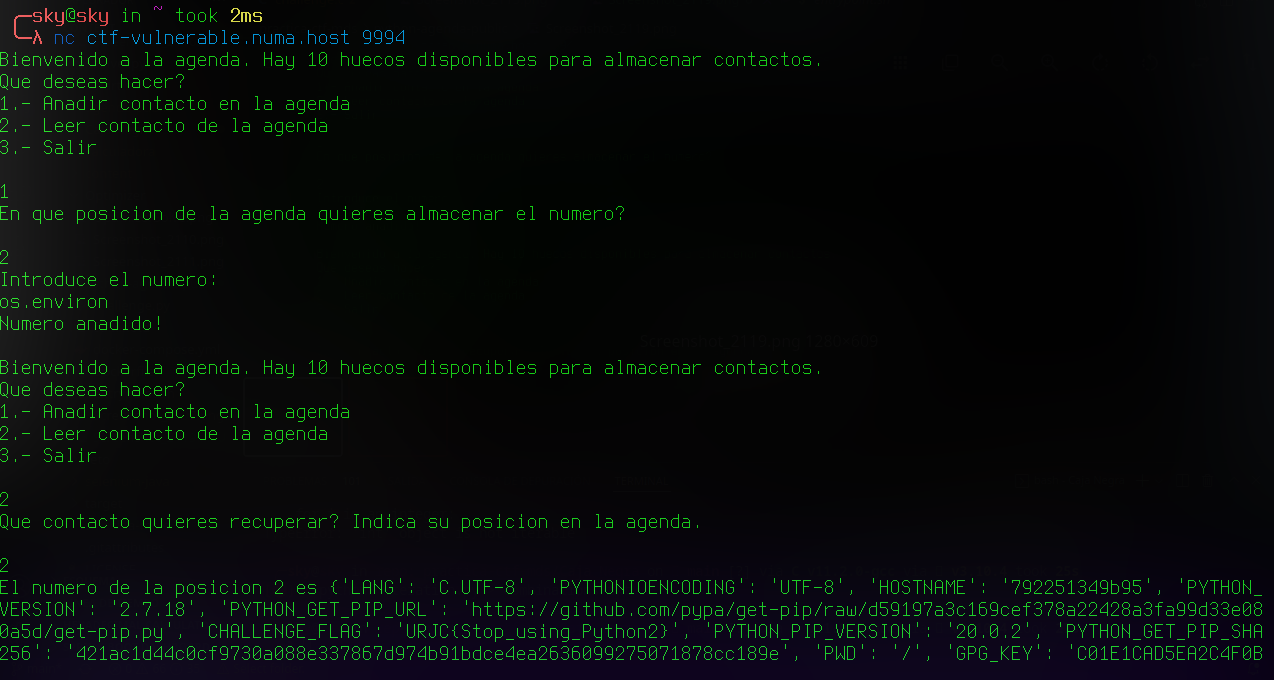
\includegraphics[width=1\linewidth]{Figuras/Agenda2/agenda2.png}
    \caption{Flag}
    \label{fig:my_label}
\end{figure}

\newpage
\section{Whack-a-mole}

Nos encontramos con el siguiente enunciado:\\

\textbf{Tenemos una infección de topos, ayúdame a acabar con ella.
\\
Nota: No es necesario un servidor remoto en este reto, la flag está oculta en el código fuente y se revela bajo ciertas circunstancias. No recomiendo hacer reversing}
\\

El html inicial muestra el siguiente tablero:
\begin{figure}[H]
    \centering
    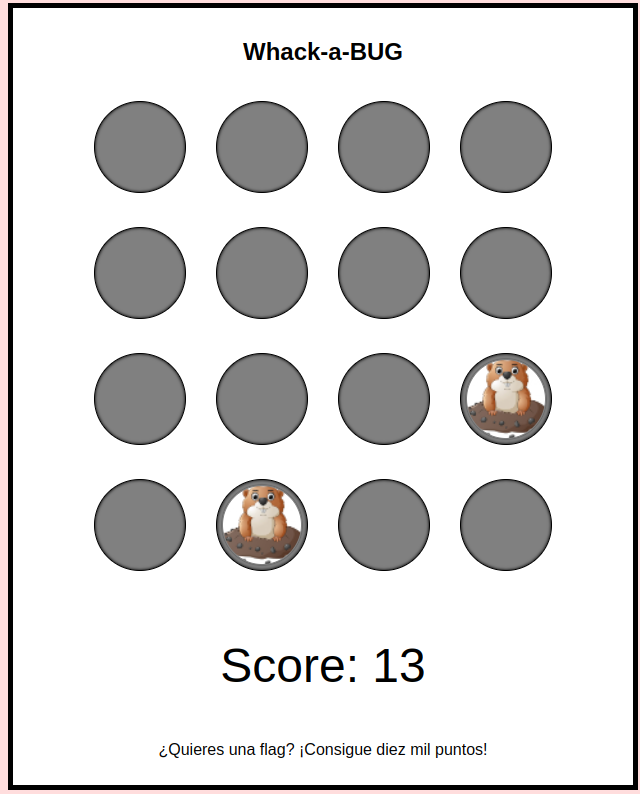
\includegraphics[width=70mm]{Figuras/WhackAMole/Inicio.png}
    \caption{Inicio}
    \label{fig:my_label}
\end{figure}

Procedemos a desarrollar un programa con Selenium en Python para automatizar el proceso:

\begin{minted}[linenos]{python}
from selenium import webdriver
from selenium.webdriver.common.by import By

driver = webdriver.Chrome()
driver.get("file:///route/to/whack-a-mole/index.html")

while True:
    try:
        mole = driver.find_element(By.CLASS_NAME, "mole")
        mole.click()
    except Exception:
        pass
\end{minted}

En primer lugar, seleccionamos el navegador que vamos a utilizar y abrimos la ruta del archivo local. Después, en un bucle infinito hacemos click en los elementos que en el html tengan como nombre de clase \emph{mole}. Podría haberse hecho con un bucle finito también.
\\
Capturamos las excepciones y las desechamos ya que python tiene un tiempo de ejecución mayor al esperado, lo que provoca excepciones.
\\
Ejecutamos y dejamos actuar el programa hasta conseguir 10000 puntos:

\begin{figure}[H]
    \centering
    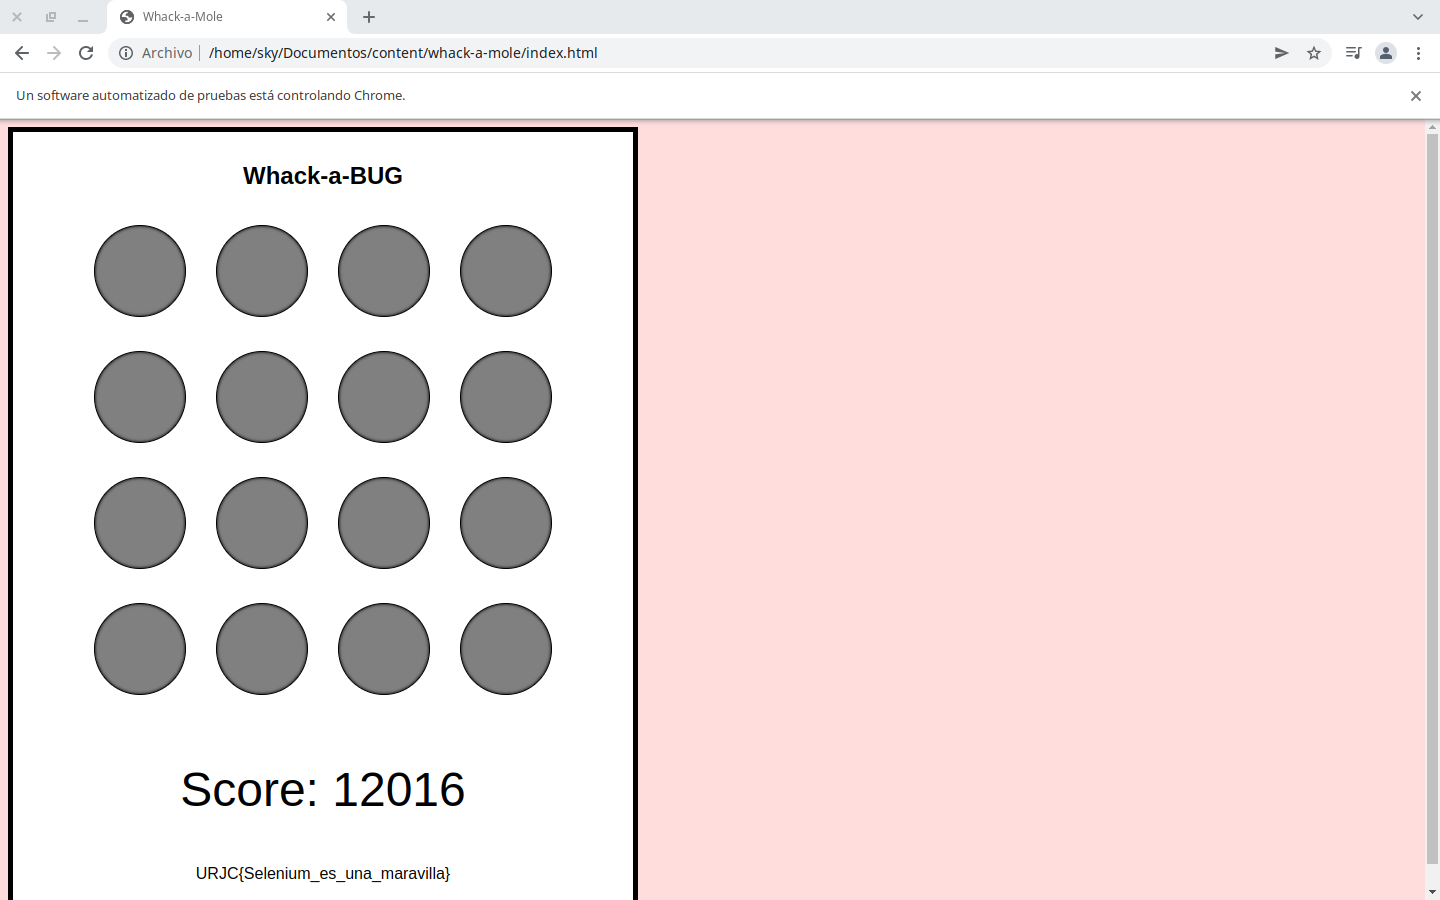
\includegraphics[width=1\linewidth]{Figuras/WhackAMole/Solucion.png}
    \caption{Flag}
    \label{fig:my_label}
\end{figure}

\newpage

\section{10 fast fingers}

Nos encontramos con el siguiente enunciado:\\
\textbf{¿Cómo de rápido escribes? ¿Eres capaz de escribir todo el texto en 5 segundos?}\\

Además se proporciona el código de la web.\\

\subsection{Método 1}

En primer lugar utilizamos un desofuscador de código online y desofuscamos el archivo app.js. Con una búsqueda de la cadena \emph{URJC}, hallamos la flag:

\begin{figure}[H]
    \centering
    \includegraphics[width=1\linewidth]{Figuras/10FastFingers/Flag.png}
    \caption{Flag}
    \label{fig:my_label}
\end{figure}

\subsection{Método 2}

La segunda forma de obtener la flag es automatizando la escritura del texto dado en el cuadro de entrada con Selenium.

\begin{figure}[H]
    \centering
    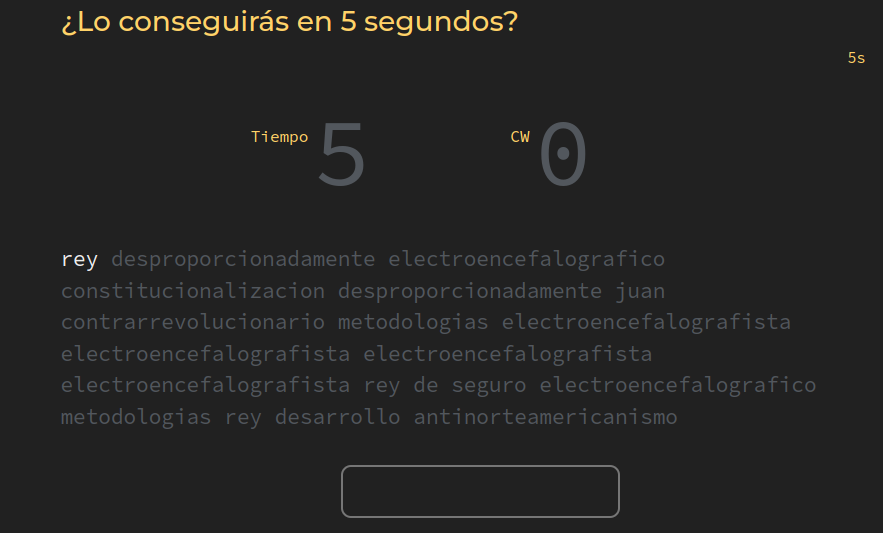
\includegraphics[width=1\linewidth]{Figuras/10FastFingers/Init.png}
    \caption{Flag}
    \label{fig:my_label}
\end{figure}

Para ello desarrollamos el siguiente código:

\begin{minted}[linenos]{Python}
from selenium import webdriver
from selenium.webdriver.common.by import By

driver = webdriver.Chrome()
driver.get("file:///route/to/reto/index.html")

try:
    elements = driver.find_elements(By.CLASS_NAME, "text-display")
    cuadro = driver.find_element(By.CLASS_NAME,"text-input")

    for i in elements:
        cuadro.send_keys(i.text)

except Exception:
    pass
\end{minted}

En éĺ, abrimos con el navegador escogido el archivo del reto y capturando las posibles excepciones y desechándolas como hemos hecho previamente, buscamos el texto por su clase. Como cada palabra tiene una clase diferente, almacenamos los elementos de la clase que lo abarca en una lista y la recorremos, escribiendo su contenido con la función \emph{send\_keys} en el cuadro de texto encontrado previamente gracias a su nombre de clase.

\\

Ejecutamos el archivo y obtenemos la flag:

\begin{figure}[H]
    \centering
    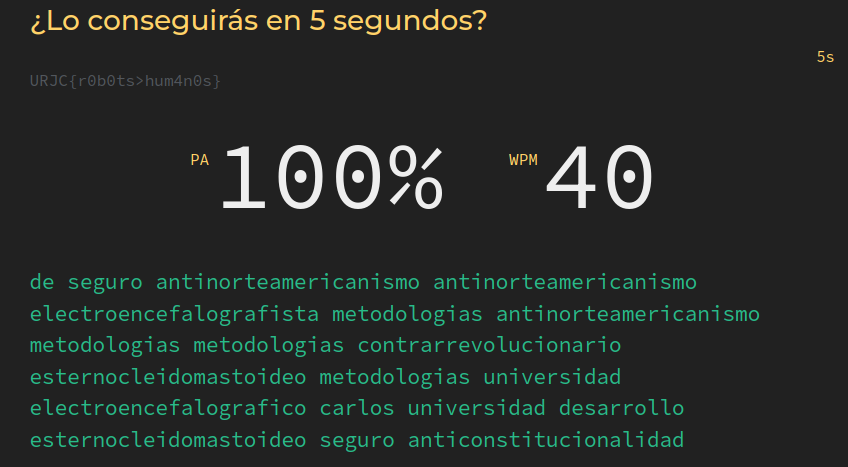
\includegraphics[width=1\linewidth]{Figuras/10FastFingers/FlagSel.png}
    \caption{Flag}
    \label{fig:my_label}
\end{figure}

\newpage

\section{Blog}

Nos encontramos con el siguiente enunciado:
\\
\textbf{Hemos descubierto un blog y nos interesa ver los temas más citados, en específico nos gustaría ver cuántas apariciones de URJC existen en todas las páginas.
\\
El blog se encuentra en -> http://ctf-vulnerable.numa.host:8040/
\\
¿Podrías ayudarme?
\\
La flag tiene el formato URJC{N}, siendo N el número de apariciones, por ejemplo: URJC{0}
\\
Nota: URJC es lo que se busca, no urjc, UrJc, etc.
\\
http://ctf-vulnerable.numa.host:8040/}\\

\vspace{4mm}

Procedemos a desarrollar un código Selenium en Python para automatizar el proceso de búsqueda.

\begin{minted}[linenos]{python}
from selenium import webdriver
from selenium.webdriver.common.by import By
import re
import time

def visita(enlaces, pattern, count, visitadas):
    try:
        enlaces = driver.find_elements(By.CLASS_NAME, 'card-title')

        for i in enlaces:
            enlace = i.find_element(By.CSS_SELECTOR,'a')
                .get_attribute('href')
        
            if enlace not in visitadas and'#' not in enlace and enlace
            .startswith('http://ctf-vulnerable.numa.host:8040/notice'):
                        
                driver.get(enlace)
                visitadas.add(enlace)
                text = driver.find_element(By.CLASS_NAME, 'article-post')
                .text
                results = re.findall(pattern, text)

                for match in results:
                    count = count + 1

            else:
            return count + visita(enlaces, pattern, count, visitadas)
            
    except Exception:
        pass

driver = webdriver.Chrome()
driver.get("http://ctf-vulnerable.numa.host:8040/") 

total = int()
enlace = driver
pattern = "URJC"
count = int = 0
visitadas = set()
enlaces = []

print(visita(enlaces, pattern, count, visitadas))
\end{minted}

Como en el challenge anterior, capturamos las excepciones y las desechamos.\\

\vspace{4mm}

En el main del programa tenemos las siguientes instrucciones:

\begin{minted}[linenos]{python}
driver = webdriver.Chrome()
driver.get("http://ctf-vulnerable.numa.host:8040/") 

pattern = "URJC"
count = 0
visitadas = set()
enlaces = []

print(visita(enlaces, pattern, count, visitadas))
\end{minted}

En primer lugar abrimos el navegador elegido con la url del blog.\\ Después establecemos los valores que nos van a permitir buscar la palabra \emph{URJC} de forma recursiva: pattern (String del patrón buscado), count (contador de la cantidad de apariciones del patrón), visitadas (para evitar entrar más de una vez a cada página) y enlaces (donde se almacenarán los enlaces contenidos en una página para ir iterando sobre ellos).

\vspace{4mm}

Por último, imprimimos el resultado de la función recursiva.\\

\newpage

Analicemos ahora la función recursiva:

\begin{minted}[linenos]{python}
def visita(enlaces, pattern, count, visitadas):
    try:
        enlaces = driver.find_elements(By.CLASS_NAME, 'card-title')

        for i in enlaces:
            enlace = i.find_element(By.CSS_SELECTOR,'a')
                .get_attribute('href')
        
            if enlace not in visitadas and'#' not in enlace and enlace
            .startswith('http://ctf-vulnerable.numa.host:8040/notice'):

                driver.get(enlace)
                visitadas.add(enlace)
                text = driver.find_element(By.CLASS_NAME, 'article-post')
                .text
                results = re.findall(pattern, text)

                for match in results:
                    count = count + 1

            return count + visita(enlaces, pattern, count, visitadas)
            
    except Exception:
        pass
\end{minted}

En primer lugar, buscamos todos los elementos de clase \emph{card-title}, ya que en estos está contenido el enlace a otras entradas del blog. Después, con un for, recorremos esa lista obteniendo el enlace contenido en el elemento, buscando el selector a y su atributo href, pues hemos observado en el html que el enlace está contenido en ese lugar.\\

Para cada elemento de la lista comprobamos si no ha sido visitado y si es un enlace de entrada de blog válido, en ese caso accedemos al enlace y lo añadimos al set de páginas visitadas. Una vez accedido al enlace, buscamos el cuerpo del blog identificado en el html con la clase \emph{article-post} y obtenemos su contenido.\\

Con el texto almacenado en una variable utilizamos regex para encontrar la cantidad de apariciones del patrón en el mismo.\\

Una vez acabado este proceso, hacemos la llamada recursiva.\\

\\

Ejecutamos el archivo obteniendo un recuento de 300 apariciones del patrón \emph{"URJC"}.

\clearpage

\end{document}
